Для того чтобы охарактеризовать степень влияния микролинзирования на кривые блеска SN Refsdal, необходимо оценить параметры галактики-линзы, ответственной за появление изображений S1-S4, а именно локальные значения параметров $\kappa_*, \kappa_c$ и $\gamma$ в областях изображений S1-S4  (см. Рис. \ref{fig:snrefsdalfig}). 

Параметры $\kappa$ и $\gamma$ известны из модели скопления MACSJ1149.6+2223 (\cite{treu2015}, а также ссылки в ней; \cite{hubblemaps}). Здесь и далее мы будем придерживаться модели\footnote{Mодели размещены на сайте stsci.edu, \cite{hlsp}.}, подробно описанной в работе \cite{kawamataoguri}. Используемые значения $\kappa$ и $\gamma$ для изображений S1-S4 приведены в Табл. \ref{tab:kappagamma}.

\begin{table}[h!]
  \caption{$\kappa$, $\gamma$ в областях изображений SN Refsdal}
  \label{tab:kappagamma}
  \centering
    \begin{tabular}{ | c | c | c | c | c |}
    \hline
    Изображение & S1 & S2 & S3 & S4 \\ \hline
    $\kappa$ & 0.728 & 0.725 & 0.670 & 0.744 \\ \hline
    $\gamma$ & 0.108 & 0.347 & 0.221 & 0.484 \\
    \hline
    \end{tabular}
\end{table}
\\
Т.к. в качестве галактики-линзы, ответственной за появление изображений S1-S4, выступает эллиптическая галактика, то оценка $\kappa_*$, то есть вклада в микролинзирование именно звёзд, может быть получена на основе эмпирических корреляций между основными свойствами эллиптических галактик: эффективным радиусом $r_e$, эффективной поверхностной плотностью звёзд $\Sigma_e$ и дисперсией скоростей звёзд $\sigma$. Эта зависимость известна как \textit{фундаментальная плоскость} (\cite{djorgovski&davis1987}, \cite{hydebernardi2009}). Также известно, что для эллиптических галактик поверхностная яркость (а значит, и поверхностная плотность звёзд) связана с расстоянием от её центра по закону де Вокулёра (\cite{vaucouleurs}).

Для оценки $\kappa_*$ и $\kappa_c$ в областях изображений сверхновой Рефсдала мы следуем подходу, детально описанному в работе \cite{schechter2014}, суть которого состоит в том, что фундаментальная плоскость записывается в терминах эффективной поверхностной плотности $\Sigma_{e}$, эффективного радиуса $r_e$ и дисперсии скоростей звёзд в галактике-линзе, которая определяется следующим образом:

\begin{equation}\label{sigsig}
\log \Sigma_{e}=A \log \left(\frac{\sigma_{p r o x}}{265  \mathrm{km} / \mathrm{s}}\right)+C,
\end{equation}

\begin{equation}\label{radeff}
\log r_{e}=D \log \left(\frac{\sigma_{\text {prox}}}{265 \mathrm{km} / \mathrm{s}}\right)+E,
\end{equation}

\begin{equation}\label{sigmaprox}
 \ \sigma_{prox}=c \sqrt{\frac{\theta_{\text {Ein}}}{4 \pi} \frac{D_{ds}}{D_{s}}},
\end{equation}
где $\theta_{\text {Ein}}$ -- радиус Эйнштейна для линзирующей галактики. Для галактик-линз на красном смещении $z \sim 0.2$ путём интерполяции данных из обзора SLACS получены значения коэффициентов (\cite{schechter2014}): $$ A = -1.702, \ C = 9.156, \ D = 2.401, \ E = 0.832. $$ Несмотря на то, что галактика, ответственная за появление изображений S1-S4 SN Refsdal, находится на $z \sim 0.5$, существенной эволюции этих параметров не ожидается. 


Поскольку значение $\theta_{\text {Ein}}$ неизвестно, воспользуемся следующим значением дисперсии скоростей звёзд для галактики-линзы: $\sigma = 232.08$ (\cite{kawamataoguri}). Ожидается, что оно лежит достаточно близко к $\sigma_{prox}$. Подставляя указанное  значение $\sigma$ в формулы \eqref{sigsig} и \eqref{radeff}, получаем: $$\Sigma_e = 1.8 \cdot 10^9 \ M_{\odot}/pc^2,$$ $$r_e=4.93 \ kpc$$
В работе \cite{kawamataoguri} приведены положения (в системе небесных координат) изображений S1-S4 (Таблица А4) и центра линзирующей галактики (раздел 3.4.4), они указаны в таблице \ref{tab:coord}.

\begin{table}[h!]
  \caption{Координаты изображений SN Refsdal и линзирующей галактики из \cite{kawamataoguri}}
  \label{tab:coord}
  \centering
    \begin{tabular}{ | c | c | c | c | c |}
    \hline
     & Прямое восхождение & Склонение \\ \hline
    S1 & 177.398225 & 22.395628 \\ \hline
    S2 & 177.397713 & 22.395781 \\\hline
    S3 & 177.397371 & 22.395531 \\ \hline
    S4 & 177.3978   & 22.395181 \\\hline
    Галактика-линза & 177.397842 & 22.395591 \\\hline
    \end{tabular}
\end{table}
\\
Поверхностная плотность звёзд $\Sigma_*$ в областях, соответствующим изображениям S1-S4, рассчитывается на основе формулы де Вокулёра (\cite{vaucouleurs}), представленной в виде (\cite{schechter2014}, формула (11)):

\begin{equation}\label{vaucouleurs}
\Sigma_*\left(u_{i}, v_{i}\right)=\mathcal{F} \frac{\Sigma_{e}}{3.607} \exp \left[-\left(\frac{w_{i}}{r_{e}}\right)^{\frac{1}{4}}+1\right], 
\end{equation}
где $u_{i}, v_{i}$ - координаты $i$-ого изображения по отношению к центру линзирующей галактики, $\Sigma_e$ - средняя (эффективная) поверхностная плотность звёзд, заключённых внутри эффективного радиуса $r_e$, безразмерный множитель $\mathcal{F}=1.23$ подобран методом максимального правдоподобия по наблюдаемым световым потокам от квазаров. При этом, согласно формуле \eqref{sigmacrit} для плоскости, в которой находятся изображения SN Refsdal  $\Sigma_{crit} = 2371.9 \ M_{\odot}/pc^2 $. Располагая этим значением, можно также найти $\kappa_*$ и $\kappa_c$ для областей с изображениями S1-S4 ($\kappa_*=\Sigma_* /\Sigma_{crit}, \ \kappa_c = \kappa-\kappa_* $). Полученные результаты представлены в таблице \ref{tab:params}.

\begin{table}[H]
  \caption{Оценки параметров для изображений SN Refsdal}
   \label{tab:params}
  \centering
    \begin{tabular}{ | c | c | c | c | c |}
    \hline
    Изображение & S1 & S2 & S3 & S4 \\ \hline
    $\Sigma_*, M_{\odot}/pc^2$ & 491.2 & 541.3 & 509.8 & 580.1\\ \hline
    $\kappa_*$ & 0.207 &  0.228 & 0.215 & 0.245 \\ \hline
    $\kappa_c$ & 0.521 & 0.496 & 0.455 & 0.499 \\ \hline
   % $\kappa_*/\kappa$ & 0.285 & 0.315 & 0.321 & 0.329 \\ \hline
    \end{tabular}
\end{table}
\\
Реализации карт с соответствующими параметрами приведены на Рисунке \ref{fig:s1s4}.

\begin{figure}[H]
    \centering
	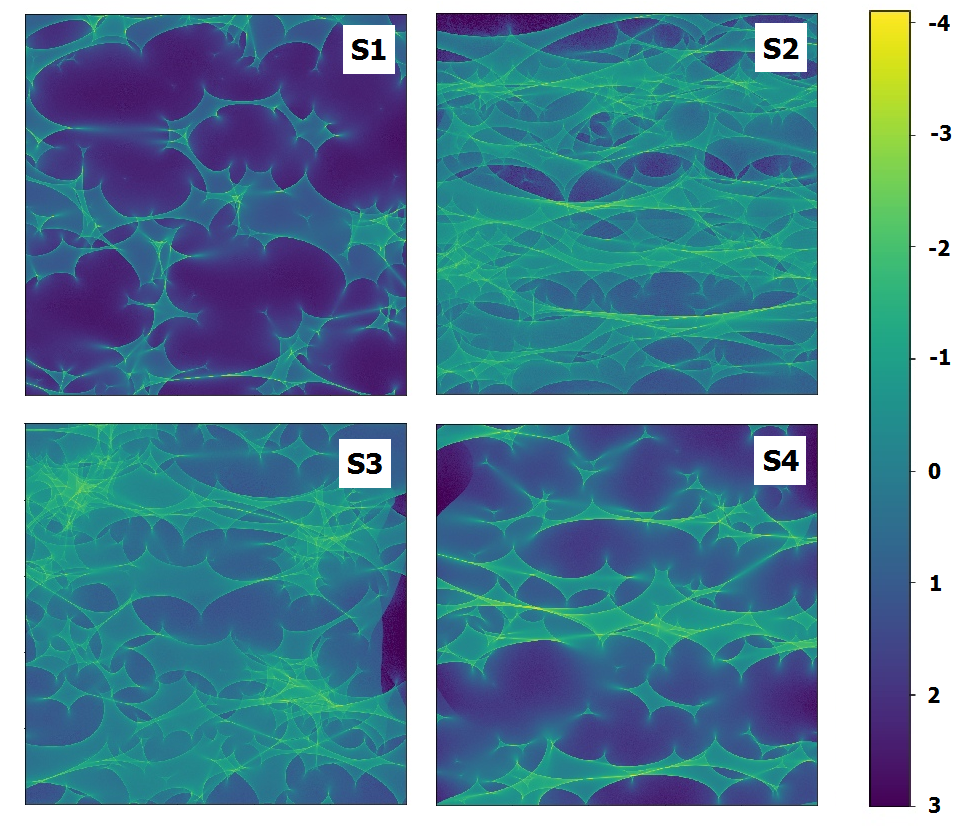
\includegraphics[scale=0.6]{pics/s1s4.png}
	\caption{Реализации карт для областей изображений S1-S4 SN Refsdal, выполненные при помощи программы {\tt{microlens}}. Размер каждой карты -- $10 \times 10 \ R_{Ein} $, разрешение -- $1000 \times 1000 $ пикселей. Цветовая шкала в единицах звёздных величин показывает усиление (отрицательные значения) или ослабление (положительные значения) яркости источника вследствие только микролинзирования. \label{fig:s1s4}} 
\end{figure}
